\documentclass[14pt]{extbook}
\usepackage{multicol, enumerate, enumitem, hyperref, color, soul, setspace, parskip, fancyhdr} %General Packages
\usepackage{amssymb, amsthm, amsmath, bbm, latexsym, units, mathtools} %Math Packages
\everymath{\displaystyle} %All math in Display Style
% Packages with additional options
\usepackage[headsep=0.5cm,headheight=12pt, left=1 in,right= 1 in,top= 1 in,bottom= 1 in]{geometry}
\usepackage[usenames,dvipsnames]{xcolor}
\usepackage{dashrule}  % Package to use the command below to create lines between items
\newcommand{\litem}[1]{\item#1\hspace*{-1cm}\rule{\textwidth}{0.4pt}}
\pagestyle{fancy}
\lhead{Progress Quiz 4}
\chead{}
\rhead{Version B}
\lfoot{6286-1986}
\cfoot{}
\rfoot{Fall 2020}
\begin{document}

\begin{enumerate}
\litem{
First, find the equation of the line containing the two points below. Then, write the equation as $ y=mx+b $ and choose the intervals that contain $m$ and $b$.\[ (9, -9) \text{ and } (10, 3) \]\begin{enumerate}[label=\Alph*.]
\item \( m \in [11, 16] \hspace*{3mm} b \in [-11, -6] \)
\item \( m \in [11, 16] \hspace*{3mm} b \in [-124, -114] \)
\item \( m \in [-13, -10] \hspace*{3mm} b \in [119, 127] \)
\item \( m \in [11, 16] \hspace*{3mm} b \in [-19, -15] \)
\item \( m \in [11, 16] \hspace*{3mm} b \in [115, 119] \)

\end{enumerate} }
\litem{
Write the equation of the line in the graph below in Standard form $Ax+By=C$. Then, choose the intervals that contain $A, B, \text{ and } C$.
\begin{center}
    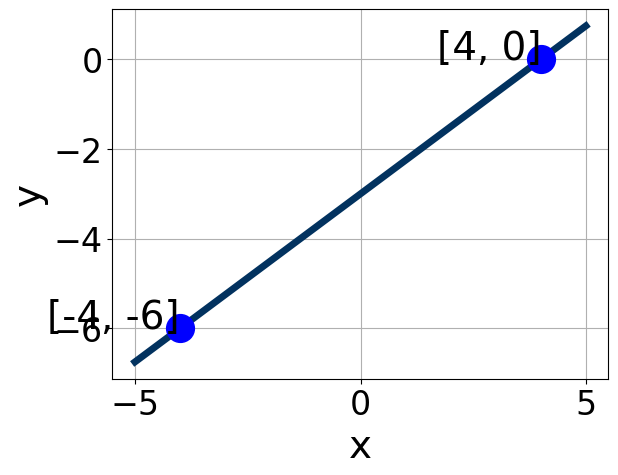
\includegraphics[width=0.5\textwidth]{../Figures/linearGraphToStandardCopyB.png}
\end{center}
\begin{enumerate}[label=\Alph*.]
\item \( A \in [1.6, 5.1], \hspace{3mm} B \in [4, 7.7], \text{ and } \hspace{3mm} C \in [-5.2, -2.8] \)
\item \( A \in [1.6, 5.1], \hspace{3mm} B \in [-6.5, -3.6], \text{ and } \hspace{3mm} C \in [4.7, 5.2] \)
\item \( A \in [-0.8, 1.3], \hspace{3mm} B \in [-0.1, 1.2], \text{ and } \hspace{3mm} C \in [-2.1, 0.7] \)
\item \( A \in [-6.7, -1.3], \hspace{3mm} B \in [-6.5, -3.6], \text{ and } \hspace{3mm} C \in [4.7, 5.2] \)
\item \( A \in [-0.8, 1.3], \hspace{3mm} B \in [-1.1, 0.2], \text{ and } \hspace{3mm} C \in [-0.2, 1.9] \)

\end{enumerate} }
\litem{
First, find the equation of the line containing the two points below. Then, write the equation as $ y=mx+b $ and choose the intervals that contain $m$ and $b$.\[ (-8, 11) \text{ and } (-4, 5) \]\begin{enumerate}[label=\Alph*.]
\item \( m \in [-3.5, 0.5] \hspace*{3mm} b \in [8.4, 9.2] \)
\item \( m \in [-3.5, 0.5] \hspace*{3mm} b \in [-0.2, 2.3] \)
\item \( m \in [-3.5, 0.5] \hspace*{3mm} b \in [16, 19.8] \)
\item \( m \in [-3.5, 0.5] \hspace*{3mm} b \in [-1.1, 0.2] \)
\item \( m \in [1.5, 6.5] \hspace*{3mm} b \in [9.9, 12.4] \)

\end{enumerate} }
\litem{
Solve the equation below. Then, choose the interval that contains the solution.\[ -9(-17x -19) = -15(-8x -5) \]\begin{enumerate}[label=\Alph*.]
\item \( x \in [-1.9, 1.1] \)
\item \( x \in [-10.45, -6.45] \)
\item \( x \in [7.45, 8.45] \)
\item \( x \in [-4.91, -0.91] \)
\item \( \text{There are no real solutions.} \)

\end{enumerate} }
\litem{
Solve the equation below. Then, choose the interval that contains the solution.\[ -3(13x -4) = -5(19x + 15) \]\begin{enumerate}[label=\Alph*.]
\item \( x \in [-1.19, -0.83] \)
\item \( x \in [-0.58, -0.22] \)
\item \( x \in [-1.79, -1.37] \)
\item \( x \in [0.89, 1.13] \)
\item \( \text{There are no real solutions.} \)

\end{enumerate} }
\litem{
Solve the linear equation below. Then, choose the interval that contains the solution.\[ \frac{4x -8}{3} - \frac{7x -5}{4} = \frac{8x + 7}{8} \]\begin{enumerate}[label=\Alph*.]
\item \( x \in [-0.5, 1.7] \)
\item \( x \in [-2.7, -0.6] \)
\item \( x \in [-3.5, -2.1] \)
\item \( x \in [-9.6, -5.5] \)
\item \( \text{There are no real solutions.} \)

\end{enumerate} }
\litem{
Find the equation of the line described below. Write the linear equation as $ y=mx+b $ and choose the intervals that contain $m$ and $b$.\[ \text{Perpendicular to } 9 x + 5 y = 8 \text{ and passing through the point } (6, -9). \]\begin{enumerate}[label=\Alph*.]
\item \( m \in [0.05, 1] \hspace*{3mm} b \in [-15.8, -14] \)
\item \( m \in [1.42, 2.17] \hspace*{3mm} b \in [-13.8, -9.4] \)
\item \( m \in [0.05, 1] \hspace*{3mm} b \in [-13.8, -9.4] \)
\item \( m \in [0.05, 1] \hspace*{3mm} b \in [12, 13.1] \)
\item \( m \in [-1.63, 0.2] \hspace*{3mm} b \in [-8.6, -4.1] \)

\end{enumerate} }
\litem{
Find the equation of the line described below. Write the linear equation as $ y=mx+b $ and choose the intervals that contain $m$ and $b$.\[ \text{Parallel to } 8 x - 5 y = 9 \text{ and passing through the point } (8, 6). \]\begin{enumerate}[label=\Alph*.]
\item \( m \in [1.23, 2.72] \hspace*{3mm} b \in [5.8, 9.8] \)
\item \( m \in [1.23, 2.72] \hspace*{3mm} b \in [-9.8, -5.8] \)
\item \( m \in [0.08, 0.75] \hspace*{3mm} b \in [-9.8, -5.8] \)
\item \( m \in [-1.95, -0.76] \hspace*{3mm} b \in [16.8, 21.8] \)
\item \( m \in [1.23, 2.72] \hspace*{3mm} b \in [-3, 3] \)

\end{enumerate} }
\litem{
Solve the linear equation below. Then, choose the interval that contains the solution.\[ \frac{-5x -9}{6} - \frac{-4x + 4}{3} = \frac{9x + 9}{5} \]\begin{enumerate}[label=\Alph*.]
\item \( x \in [-4.09, -2.67] \)
\item \( x \in [-1.22, -0.29] \)
\item \( x \in [-17.54, -16.44] \)
\item \( x \in [-1.83, -1.14] \)
\item \( \text{There are no real solutions.} \)

\end{enumerate} }
\litem{
Write the equation of the line in the graph below in Standard form $Ax+By=C$. Then, choose the intervals that contain $A, B, \text{ and } C$.
\begin{center}
    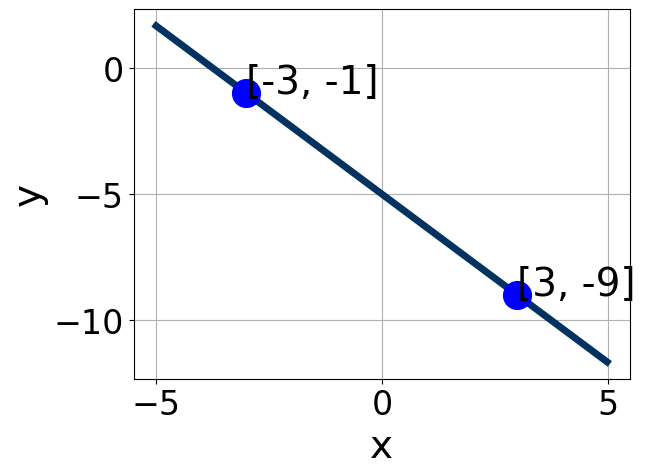
\includegraphics[width=0.5\textwidth]{../Figures/linearGraphToStandardB.png}
\end{center}
\begin{enumerate}[label=\Alph*.]
\item \( A \in [2.84, 4.19], \hspace{3mm} B \in [1.27, 2.29], \text{ and } \hspace{3mm} C \in [-6.5, -4.8] \)
\item \( A \in [1.08, 2.37], \hspace{3mm} B \in [0.59, 1.23], \text{ and } \hspace{3mm} C \in [-3.1, -2.6] \)
\item \( A \in [-3.32, -2.01], \hspace{3mm} B \in [-2.44, -1.82], \text{ and } \hspace{3mm} C \in [5.9, 7.3] \)
\item \( A \in [2.84, 4.19], \hspace{3mm} B \in [-2.44, -1.82], \text{ and } \hspace{3mm} C \in [5.9, 7.3] \)
\item \( A \in [1.08, 2.37], \hspace{3mm} B \in [-1.32, -0.95], \text{ and } \hspace{3mm} C \in [1.1, 3.2] \)

\end{enumerate} }
\end{enumerate}

\end{document}